% Original manuscript following the SoftwareX Original Software Publication
% template retrieved 2026-09-26 from:
% https://legacyfileshare.elsevier.com/promis_misc/softwarex-osp-template.tex
% The template's document class, paper size, font size and five sections are retained.
% This is an author-review draft, not a claim of submission or acceptance.
\documentclass[preprint,12pt,a4paper]{elsarticle}

\usepackage[T1]{fontenc}
\usepackage{iftex}
\ifPDFTeX
	\usepackage[utf8]{inputenc}
\fi
\usepackage{amsmath,amssymb}
\usepackage{booktabs,tabularx,array}
\usepackage{xcolor}
\usepackage{xurl}
\usepackage{hyperref}
\hypersetup{hidelinks,pdftitle={osm-accessibility-research: Auditable preference-aware pedestrian routing on OpenStreetMap graphs},pdfauthor={Alex Martinelli}}
\setlength{\parindent}{0pt}
\newcommand{\software}{\texttt{osm-\allowbreak accessibility-\allowbreak research}}
\newcommand{\CodeVersion}{0.3.0}
\newcommand{\CodeCommit}{b3d2076689725777b4581e36a5c9ce7d12c507ae}
\newcommand{\AuthorQuery}[1]{\textcolor{red!65!black}{\textbf{[AUTHOR INPUT: #1]}}}
\newcommand{\Pending}{\textcolor{red!65!black}{\textit{Pending}}}
\newcolumntype{Y}{>{\raggedright\arraybackslash}X}
\journal{SoftwareX}

\begin{document}
\begin{frontmatter}
\title{osm-accessibility-research: Auditable preference-aware pedestrian routing on OpenStreetMap graphs}
\author[fau]{Alex Martinelli\corref{corresponding}}
\ead{alex.martinelli@fau.de}
\cortext[corresponding]{Corresponding author.}
\address[fau]{M.Sc. Data Science, Friedrich-Alexander-Universit\"at Erlangen-N\"urnberg (FAU), Erlangen, Germany}

\begin{abstract}
Accessibility-aware routing studies need reproducible comparisons of routes.
We present
\software{}, a Python toolkit for pedestrian routing on OpenStreetMap graphs.
It separates hard rules from preference penalties, and continuous attributes
from arrival-node events. Selected routes are compared with a
no-preference shortest route under a common assessment profile, with infeasible
alternatives and missing information reported explicitly. Exact route traces,
criterion-level diagnostics and provenance accompany corridor-focused figures.
A deterministic example and automated regression tests demonstrate the
computational workflow. The software supports inspectable scenario analysis,
not certified navigation: its scores describe a specified model rather than
measured accessibility or safety.
\end{abstract}

\begin{keyword}
OpenStreetMap \sep Pedestrian routing \sep Accessibility \sep Research software
\sep Reproducibility \sep Geospatial analysis
\end{keyword}
\end{frontmatter}

\noindent\AuthorQuery{Review draft. Insert the Erlangen study, approve declarations,
select the code license, and confirm the full affiliation/postal address before submission.}

\clearpage
\section*{Required Metadata}
\section*{Current code version}
\begin{table}[!ht]
\small
\begin{tabularx}{\textwidth}{@{}p{0.052\textwidth}>{\raggedright\arraybackslash}p{0.36\textwidth}Y@{}}
\toprule
\textbf{Nr.} & \textbf{Code metadata description} & \textbf{Value} \\
\midrule
C1 & Current code version & \CodeVersion{}; scientific code revision \texttt{b3d2076}. \\
C2 & Permanent GitHub link to code/repository used for this code version &
\url{https://github.com/AlexM3020/accessible-routing-openstreetmap/tree/b3d2076689725777b4581e36a5c9ce7d12c507ae} \\
C3 & Legal Code License & \AuthorQuery{No code license is declared at the documented revision. Choose an approved open-source license and add the required license file before submission.} \\
C4 & Code versioning system used & Git. \\
C5 & Software code languages, tools, and services used & Python; Matplotlib; pyproj/PROJ; Shapely/GEOS. Command-line interface and importable modules; optional MongoDB snapshot storage. \\
C6 & Compilation requirements, operating environments \& dependencies & Python $\geq$3.11; pymongo $\geq$4.10,$<$5; Matplotlib $\geq$3.9,$<$4; pyproj $\geq$3.6,$<$4; Shapely $\geq$2.0,$<$3; defusedxml $\geq$0.7,$<$1; ijson $\geq$3.3,$<$4. GEOS $\geq$3.10 is required for distance predicates. Local validation: Windows, Python 3.12.10. Dependencies may require platform-specific wheels or libraries. \\
C7 & If available Link to developer documentation/manual &
\href{https://github.com/AlexM3020/accessible-routing-openstreetmap/blob/b3d2076689725777b4581e36a5c9ce7d12c507ae/README.md}{Version-specific GitHub README}; runnable example and tests in the same revision. \\
C8 & Support email for questions & \href{mailto:alex.martinelli@fau.de}{alex.martinelli@fau.de} \\
\bottomrule
\end{tabularx}
\caption{Code metadata. The software revision is fixed independently of subsequent manuscript edits. The unresolved license is a submission blocker, not a license grant.}
\label{tab:metadata}
\end{table}
\clearpage

\section{Motivation and significance}
\label{sec:motivation}
The shortest mapped pedestrian route need not suit a particular traveller.
Stairs, kerbs, narrow paths, steep inclines and surface conditions can affect
route suitability differently across mobility requirements. OpenStreetMap (OSM)
provides a collaboratively maintained representation of these features
\cite{haklay2008}, but a missing attribute does not establish the absence of an
obstacle. Research therefore needs to explain both \emph{why a path was selected}
and \emph{which observations support that explanation}.

Personalised wheelchair routing and the reliability of volunteered geographic
information are established topics; Neis explicitly considers individual
requirements and route-data reliability \cite{neis2015}. OSMnx provides a broader
Python workflow for constructing and analysing street networks
\cite{boeing2017}. The contribution here is not a new shortest-path algorithm
or a claim of superior routing accuracy. It is a focused, inspectable software
workflow connecting a declared preference model to exact directed traces,
like-for-like assessment, missing-data disclosure and reproducible outputs.
A* \cite{hart1968} and Dijkstra's algorithm \cite{dijkstra1959} remain the search
methods.

\software{} targets researchers comparing accessibility assumptions on a fixed
OSM extract, analysts inspecting the reasons for detours, and developers testing
alternative tag interpretations. A user supplies a complete extract, two
coordinates, a profile and cost parameters. The software constructs the graph,
finds routes, assesses them and exports a compact evidence bundle. A database
and a running web service are unnecessary for this workflow. Version-specific
source and explicit provenance support software citation and reuse
\cite{smith2016,barker2022}; they do not by themselves establish complete FAIR
compliance or empirical validity.

\section{Software description}
\label{sec:software}
\subsection{Software architecture}
\label{sec:architecture}
The Python package separates ingestion, graph records, evaluation, search,
experiment orchestration and presentation (Table~\ref{tab:architecture}).
Immutable node, edge and profile records make the inputs explicit. A run-local
evaluation cache supplies costs and diagnostics consistently to search and export.
The interface exposes \texttt{demo}, \texttt{route},
\texttt{plot}, \texttt{sweep}, \texttt{query} and \texttt{import-osm}; the same
workflow can be called from Python.

\begin{table}[!ht]
\small
\begin{tabularx}{\textwidth}{@{}p{0.29\textwidth}Y@{}}
\toprule
\textbf{Layer} & \textbf{Responsibility and boundary} \\
\midrule
Ingestion and topology & Validate OSM XML/Overpass JSON and referenced nodes; construct a directed multigraph without inventing geometric intersections. \\
Profiles and evaluation & Keep hard exclusions separate from ten weighted criteria; return risk, known-data indicators and reasons. \\
Search and experiments & Snap endpoints, run A*/Dijkstra and comparison searches, preserve predecessor edges, and record provenance. \\
Outputs and visualisation & Export exact GPX, complete diagnostic tables, paired-route reports and clipped corridor figures; display settings do not change search. \\
\bottomrule
\end{tabularx}
\caption{Responsibilities of the principal software layers.}
\label{tab:architecture}
\end{table}

Edges connect consecutive OSM references; parallel edges and their way identifiers
remain distinct. Connectivity depends on shared node identifiers, not apparent
line crossings. Missing references and conflicting input records are rejected.
Pedestrian-specific direction tags control directed edges; vehicle one-way rules
are not automatically imposed on pedestrians. Requested endpoints are snapped
to eligible connected nodes, requiring an outgoing edge at the origin and an
incoming edge at the destination. The default maximum snap distance is 150~m.
Snap gaps are recorded but excluded from route distance and GPX: the software
does not assert that these off-network connections are traversable.

\subsection{Software functionalities and cost model}
\label{sec:model}
Hard restrictions exclude unsupported pedestrian highways, restricted access
and specified physical barriers. The separate \texttt{wheelchair\_required}
flag additionally rejects explicit wheelchair prohibitions, selected barrier
types without affirmative wheelchair tags, and steps without a ramp accepted
by the model. Setting a soft weight to its maximum does not create a hard
constraint. Width and incline preferences are soft penalties, not certified
clearance or gradient limits.

Ten criteria concern cycling conflicts, lighting, surface, smoothness, kerbs,
crossing control, width, incline, stairs and mapped wheelchair access.
Active weights $w_j\in(0,1]$ combine heuristic risks $r_{ej}\in[0,1]$ separately
for continuous way attributes and arrival-node events. Unrecognised or absent
observations use a configurable unknown-risk value $\rho$ and retain their
unknown status. Let $W_e$ and $T_e$ denote the respective active criterion sets.
For either set $A$, define
\begin{equation}
\overline r_e(A)=
\begin{cases}
\displaystyle\frac{\sum_{j\in A}w_jr_{ej}}{\sum_{j\in A}w_j}, & A\ne\varnothing,\\
0, & A=\varnothing.
\end{cases}
\label{eq:risk}
\end{equation}
Writing $R_e=\overline r_e(W_e)$ and $U_e=\overline r_e(T_e)$, the cost of a
permitted edge of mapped length $d_e$ is
\begin{equation}
C(e)=d_e+\lambda\bigl(d_eR_e+qU_e\bigr).
\label{eq:cost}
\end{equation}
Here $\lambda\geq0$ controls the distance--risk trade-off and $q\geq0$ is an
event-equivalent length. Defaults are $\lambda=1.5$, $q=20$~m and $\rho=0.5$.
These values are configurable modelling assumptions, not calibrated
probabilities or universal mobility thresholds. Crossing and kerb node events
are charged on arrival. Corresponding way-level criteria are suppressed when
the event is represented by relevant nodes, avoiding duplicated charges.

The scored exposure is
$E_e=d_e\mathbf{1}_{W_e\ne\varnothing}+q\mathbf{1}_{T_e\ne\varnothing}$.
For a feasible route $P$ with positive exposure, its preference match is
\begin{equation}
S(P)=100\left(1-
\frac{\sum_{e\in P}(d_eR_e+qU_e)}{\sum_{e\in P}E_e}\right),
\label{eq:score}
\end{equation}
numerically bounded to $[0,100]$. This pools exposures rather than averaging
edge percentages. Let $\kappa_e(A)$ be the fraction of active weight in $A$
whose observation is recognised, or zero for an empty set. Reported coverage is
\begin{equation}
K(P)=100\frac{\sum_{e\in P}\{d_e\kappa_e(W_e)+q\kappa_e(T_e)\}}
{\sum_{e\in P}E_e}.
\label{eq:coverage}
\end{equation}
Coverage describes recognised selected-criterion exposure, not physical
inspection coverage. Zero exposure yields no score or coverage; it does not
yield perfect accessibility. An infeasible comparison route has no comparable
match score. Unknown observations remain listed even when $\rho=0$.

Search minimises the sum of Eq.~\ref{eq:cost}. Edge lengths are checked against
endpoint Haversine distance, with a numerical tolerance, and penalties are
nonnegative. The Haversine heuristic therefore supplies an admissible lower
bound for the constructed graph to that tolerance. A* and Dijkstra target the
same scalar objective, not a Pareto frontier. Equivalent subdivision of a
uniformly tagged approach edge preserves the tested route cost, but the local
event-inclusive edge score can change when an event's exposure becomes
concentrated in a shorter incoming segment.

\subsection{Paired comparison and reproducible output}
\label{sec:comparison}
Every experiment also finds a \emph{standard route}: the shortest mapped
pedestrian distance between the same snapped endpoints, with all soft weights
zero and the wheelchair hard requirement disabled. Basic pedestrian-access,
physical-barrier and direction rules remain. Both traces are subsequently
assessed using the \emph{selected} profile and parameters. This avoids comparing
percentages produced by different measuring rules. A standard path that breaks
selected hard requirements is labelled infeasible, not recommended as an
alternative. Differences can reflect changed hard feasibility as well as soft
weights. An additional distance-only baseline retaining the selected hard
constraints separates these effects; optional A*/Dijkstra checks assess cost
agreement on the same problem.

The report distinguishes observed encounters, known selected-preference
conflicts, missing information and blocked directed traversals. Counts group
contiguous way observations or node visits; they are not stair risers or counts
of independent physical objects. One feature can occur in multiple type rows,
and nonconsecutive revisits can count again. Signed differences expose both
benefits and disadvantages. Their interpretation depends on OSM segmentation
and the selected measuring rule.

Five default files contain selected-route GPX, a readable summary, two PNG
figures and a compressed reproducibility archive. Optional vector PDF output
uses Matplotlib \cite{hunter2007}. Both figure viewports follow a default
150~m buffer around the union of the two paths in a local azimuthal-equidistant
projection. Only the displayed context is clipped; graph search and archived
diagnostics retain the full extract. Shapely's spatial index supplies exact
nearest-segment queries \cite{shapely}, avoiding a Python scan of every path
segment for every candidate marker. Marker filtering and caps never truncate
the complete comparison. Display offsets of at most 1~m expose coincident
directions in the score layer only; route traces remain unshifted.

The archive records the input snapshot, both directed traces, profile,
parameters, criterion-level diagnostics, checksums, code fingerprints and
environment information. Replotting verifies these records and uses stored
traces rather than fresh searches. The archive is written last and never
silently replaces an earlier run. Checksums detect inconsistency, not malicious
rewriting of every record; they are not digital signatures. A parameter sweep
reuses the same graph and endpoints to examine cost and missingness assumptions.

\section{Illustrative examples}
\label{sec:examples}
\subsection{Deterministic synthetic example}
\label{sec:synthetic}
The bundled \texttt{demo} fixture contains 12 nodes and 30 directed edges,
including stairs, rough and smooth alternatives, node events, a restrictive
barrier, unknown attributes and a disconnected component. Its geographic
coordinates are illustrative: the fixture is not an observed Erlangen network.
The example uses the built-in wheelchair profile, $\lambda=6$, and the other
default cost parameters. The companion figure-generation script checks the
complete implementation fingerprint against the documented revision and
derives the table and figure from an actual experiment.

\begin{table}[!ht]
\centering
\small
% Generated by paper/generate_example.py; do not hand-edit numeric results.
\begin{tabular}{@{}lrrr@{}}
\toprule Measure & Selected & Standard & Change \\
\midrule
Distance (m) & 477.8 & 144.2 & +333.6 \\
Profile match (\%) & 97.6 & \textit{Infeasible} & --- \\
Recognised-data coverage (\%) & 100.0 & 40.0 & +60.0 \\
Blocked directed traversals & 0 & 2 & -2 \\
Known soft-conflict groups & 1 & 2 & -1 \\
Unknown-observation groups & 0 & 6 & -6 \\
Stairs encounters & 0 & 1 & -1 \\
Wheelchair restriction encounters & 0 & 1 & -1 \\
Lighting encounters & 1 & 0 & +1 \\
\bottomrule
\end{tabular}

\caption{Synthetic paired-route assessment under the selected wheelchair profile.
Changes are selected minus standard. The standard route crosses a mapped
stairway and is infeasible under that profile; its score is therefore undefined.
The two blocked traversals are graph edges, not two separate stairways.
Stair and wheelchair-restriction entries describe the same tagged feature.}
\label{tab:synthetic}
\end{table}

The selected route is 477.8~m, versus 144.2~m for the standard route
(Table~\ref{tab:synthetic}). It has no stairway encounter but includes one
unlit-way encounter. Thus the comparison does not conceal an adverse lighting
trade-off. Its 97.6\% match and 100\% recognised-data coverage describe the
artificial tags only. The distance-only baseline under the same hard
requirements is 305.9~m, giving a 56.2\% selected-route distance overhead against
that feasible baseline, distinct from comparison with the unrestricted
standard. A*/Dijkstra cost agreement is checked numerically, not used as
evidence that the accessibility model is accurate.

\begin{figure}[!ht]
\centering
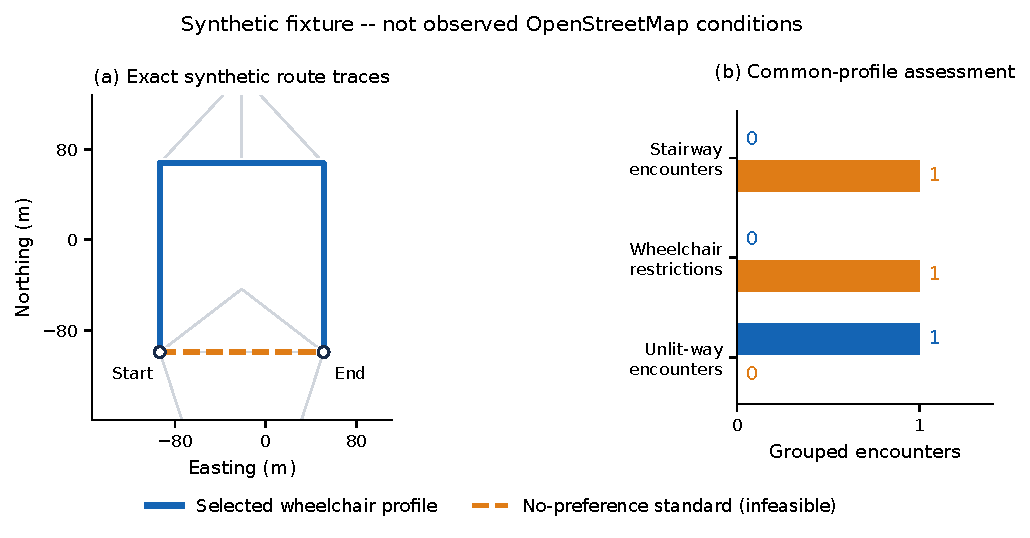
\includegraphics[width=\textwidth]{figures/synthetic-comparison.pdf}
\caption{Deterministic software output, not field data. Left: exact selected
and standard traces with context clipped to a 60~m display corridor. This
manuscript-specific radius does not affect routing; the application default is
150~m. Right: grouped known-feature encounters from the same assessment as
Table~\ref{tab:synthetic}. Counts of different types must not be summed as
independent physical obstacles. The vector figure is regenerated from the
bundled fixture, without map tiles, screenshots or generated observational imagery.}
\label{fig:synthetic}
\end{figure}

\subsection{Software verification and performance boundaries}
\label{sec:verification}
At the documented version, the automated suite records 343 passing tests and
one skip on Windows with Python 3.12.10. The skipped test requires unavailable
symbolic-link permissions. Combined statement/branch-aware coverage is
approximately 93\%, not 93\% branch coverage considered alone. Tests exercise
cost and exposure decomposition, hard exclusions, node-event handling,
coordinate conventions, exact GPX order, invalid inputs, archive tampering,
paired comparisons, corridor clipping and plotting non-mutation. Numerical
search checks use the same evaluator, so they cannot independently validate
that evaluator's assumptions. Additional checks cover lint, dependency
consistency, source compilation and installation of the built wheel outside
the source tree.

The spatial-index regression uses 4,000 candidates and 800 segments along a
synthetic 2~km path, comparing indexed distances with exhaustive geometric
distances. It tests removal of the repeated scan, not a guaranteed query-time
bound. End-to-end runtime still includes parsing, graph construction,
additional searches, full-graph diagnostics, rendering and archive writing.
Search timings exclude those stages. Development timing samples are not
presented as a representative city-scale benchmark; the Erlangen study must
report its own hardware, extract size and repeated measurements.

% Replace this subsection with the completed study, not merely a populated table.
% Keep observed field facts separate from model outputs and synthetic results.
\subsection{Erlangen, Germany: local evaluation to be completed}
\label{sec:erlangen}
\AuthorQuery{Insert the actual Erlangen study design, results and interpretation
here. No local field measurements or city-scale performance results were
provided for this draft. The following is an evaluation plan and reporting
scaffold, not a claim that these procedures have already been performed.}

The local evaluation will examine route comparisons on a fixed OSM extract
covering the selected study area in Erlangen, Germany. The report should
identify the extraction date, geographic boundary, input checksum, graph size
and any preprocessing. Origin--destination pairs should be specified using
an auditable sampling rule, rather than choosing only favourable examples.
Both successful and failed requests, including snapping failures, should be
reported. The approximately 2~km case motivating the output redesign can be
included, but its actual route, observations and timing must be supplied.

For each successful request, compare the selected route with both the
no-preference standard and the distance-only route under matched hard
constraints. Keep endpoints, input snapshot and assessment profile fixed.
Report distance, grouped feature encounters, known preference conflicts,
unknown observations, coverage and feasibility; score differences are defined
only for feasible routes under the same measuring rule. Distinguish
model-reported obstacles from independently audited physical features, using
a stated correspondence rule between audited features and OSM elements.
Audit dates, measurement methods, accessible alternatives and uncertainty
should accompany any assertion about physical suitability. Do not ask a
participant to traverse an alternative that violates their requirements merely
to complete a comparison.

Runtime evaluation should separate loading, graph construction, search,
diagnostics, figures and archive creation, and record hardware, software
versions, cold and warm conditions, repetitions and memory-measurement methods.
Summaries should retain the paired structure, state their denominators and
show variability. If repeated requests or several profiles share an
origin--destination pair, uncertainty estimates must not treat those
observations as independent without justification.

\begin{table}[!ht]
\small
\begin{tabularx}{\textwidth}{@{}>{\raggedright\arraybackslash}p{0.43\textwidth}Y@{}}
\toprule
\textbf{Required Erlangen information} & \textbf{Author-supplied result} \\
\midrule
Study boundary; extract date/hash; nodes/edges & \Pending \\
Route-pair selection; requested/successful/failed counts & \Pending \\
Profiles, hard requirements and cost parameters & \Pending \\
Independent audit method, dates and feature correspondence & \Pending \\
Paired distances, encounters, conflicts and unknowns & \Pending \\
Feasibility and common-profile scores/coverage & \Pending \\
Runtime/memory, hardware, repetitions and variability & \Pending \\
Field agreement, uncertainty and unfavourable cases & \Pending \\
Data availability, OSM attribution and privacy safeguards & \Pending \\
\bottomrule
\end{tabularx}
\caption{Placeholder for the Erlangen evaluation. ``Pending'' means no result
has been supplied; it does not mean zero, no obstacle, or a successful test.}
\label{tab:erlangen}
\end{table}

\AuthorQuery{Replace the plan with what was actually done and report the
results, including null or adverse findings. Add an appropriately attributed
Erlangen map only after choosing the real study area. If participants,
identifiable locations or personal mobility data were involved, state the
applicable ethics approval or exemption, consent and privacy arrangements;
do not claim approval or exemption without verification. Update the abstract,
impact and conclusions to reflect only the supplied evidence.}

\subsection{Companion web demonstration}
\label{sec:webdemo}
A companion interface, Roam, is linked at
\url{https://roam-um3s.onrender.com/}. It illustrates interactive preference
selection, map-based endpoints and GPX-oriented route inspection. It is a
separately deployed frontend/backend application, not a version-locked build
of this Python research package. Its live availability and data can change;
it is neither a source of the measurements above nor an archival reproduction
environment. The command-line example and frozen software revision remain the
reference execution path. Service availability must be checked before
submission; a reachable interface alone does not establish a working routing
service.

\section{Impact}
\label{sec:impact}
The principal contribution is an auditable experiment unit: a chosen path,
its alternative, the measuring rule and the evidence needed to inspect their
differences travel together. This addresses a practical weakness of reporting
only a coloured path or a single accessibility percentage. Researchers can
trace a reported difference back to a directed edge, criterion and recorded
observation, then change presentation without rerunning the searches. The
synthetic example demonstrates that workflow concretely: a shorter standard
route has a stair restriction, while the selected alternative trades distance
and lighting conditions against that restriction.

Three research uses follow. First, fixed-input sweeps can identify route
choices sensitive to weights, event-equivalent length or unknown-data risk.
Second, common-profile assessment and the matched-hard-constraint baseline
support separate questions about preference penalties and wheelchair
feasibility rules. Third, missing-data lists can guide a \emph{manual} review
of influential attributes before interpreting a favourable model score.
Automated active learning, learned preferences and empirical discomfort
prediction are not implemented. These are opportunities for subsequent work,
not capabilities attributed to the current release.

The modular package allows alternative tag rules to be investigated without
reimplementing file parsing, trace export or paired reporting. Explicit
versioning and portable tabular evidence support integration into research
workflows, consistent with the motivations behind research-software citation
and FAIR4RS \cite{smith2016,barker2022}. No independent adoption statistics,
downstream publications, commercial deployment outcomes or demonstrated
change in other users' practice are reported. Current evidence consists of
software verification and reproducible examples; the Erlangen section is
reserved for the author's independent application evidence.

Important boundaries remain. The toolkit is an in-memory regional analyser,
not a planet-scale or real-time navigation service. Completeness and currency
of OSM tags constrain what can be observed. Straight graph-node snapping,
the absence of invented intersections, and missing ramp or barrier information
can prevent a route even when a real alternative exists. Uphill and downhill
inclines have the same absolute-grade penalty, and handrail and width rules
are simplified hypotheses. Ordinary mapping omissions can make a low
encounter count misleading. Device-specific usability, temporary works and
traveller experience require independent assessment. OSM data also retain
their own attribution and ODbL obligations \cite{osmlicense}, separate from
the code's unresolved license. Accordingly, potential research utility should
not be read as demonstrated physical accessibility or universal suitability.

\section{Conclusions}
\label{sec:conclusions}
The toolkit provides an auditable workflow for preference-aware pedestrian
routing, standard-route comparison and reproducible inspection of OSM-derived
evidence. Separating feasibility, weighted risk, node events and missingness
makes the reported trade-offs interpretable. Exact traces, common-profile
assessment, focused figures and verified archives support reuse without
presenting model-generated percentages as ground truth. Automated tests and
the synthetic example establish computational behaviour within the implemented
rules. Independent Erlangen results must be added before making local
performance or accessibility claims; broader generalisation will require
additional datasets and evaluation with intended users.

\section*{Code and data availability}
The code and documentation are available at the version-specific GitHub link
in Table~\ref{tab:metadata}. The synthetic fixture is defined in the source;
the manuscript figure, table and provenance are generated by
\texttt{paper/generate\_example.py}. The Erlangen extract, measurements and
redistribution statement are pending author input in
Section~\ref{sec:erlangen}. No software or dataset DOI has been assigned in
this draft. Public source visibility does not substitute for an explicit
reuse license; the unresolved code-license entry must be completed.

\section*{CRediT authorship contribution statement}
\textbf{Alex Martinelli:} Conceptualization, Methodology, Software,
Visualization, Writing---original draft.
\AuthorQuery{Confirm these roles, add the actually performed investigation,
data curation, validation and review/editing roles, and confirm sole authorship.}

\section*{Funding}
\AuthorQuery{Supply funding sources, grant identifiers and sponsor roles, or
confirm that this research received no specific grant. No funding status has
been inferred from the affiliation.}

\section*{Declaration of competing interest}
\AuthorQuery{Supply the approved statement of competing interests, covering
financial and other interests, or explicitly confirm that there are none.}

\section*{Acknowledgements}
The work uses contributions from the OpenStreetMap community and the
maintainers of the Python scientific and geospatial dependencies cited or
listed above. \AuthorQuery{Add any individual acknowledgements with permission,
or remove this query if none are needed.}

\section*{Declaration of generative AI and AI-assisted technologies in the manuscript preparation process}
GitHub Copilot was used to assist source-code inspection, manuscript
organisation and drafting, and LaTeX preparation. It was also used during
development of the software. The synthetic figure is a deterministic plot of
software-generated fixture data; no Erlangen observations, participant data or
field results were generated. The author is responsible for the accuracy and
originality of the final article.
\AuthorQuery{Review and edit the entire draft, verify the references and all
claims, and confirm that the submitted declaration accurately describes the
tools used and the completed human review.}

\bibliographystyle{elsarticle-num}
\bibliography{references}

\section*{Current executable software version}
Version \CodeVersion{} is distributed as a Python package and command-line
entry point, not as a separately versioned binary. Installation and execution
instructions are in the version-specific repository documentation. The
companion website in Section~\ref{sec:webdemo} has a separate deployment
lifecycle and is not identified as an equivalent executable release.

\end{document}